\documentclass[11pt,a4paper]{article}
\usepackage[utf8]{inputenc}
\usepackage[T1]{fontenc}
\usepackage{amsmath,amssymb}
\usepackage{graphicx}
\usepackage{booktabs}
\usepackage{hyperref}
\usepackage[margin=1in]{geometry}

\title{County-Level Vulnerability to SNAP Participation Losses\\Under Expanded ABAWD Work Requirements}
\author{Jiaming Zhang \\ Department of Agricultural, Food, and Resource Economics \\ Michigan State University}
\date{\today}

\begin{document}
\maketitle
\begin{abstract}
I evaluate the heterogeneous effects of SNAP ABAWD work requirements across Michigan counties, using a county-month panel and Michigan's staggered 2017--2018 reinstatement of time limits. Using the Callaway--Sant'Anna estimator for staggered difference-in-differences, I estimate dynamic participation responses and characterize systematic heterogeneity across counties by unemployment, rurality, poverty, education, social vulnerability, and baseline SNAP dependence. I then translate the estimated heterogeneity into ex-ante projections of county-level participation losses under a 2026 OBBA policy expansion (age 55--64), with uncertainty intervals and alternative labor-market scenarios. The primary output is a county vulnerability ranking that identifies which local areas face the greatest risk of SNAP caseload losses, directly informing implementation planning, targeted outreach, and administrative capacity allocation.
\end{abstract}

\section{Introduction}
\label{sec:intro}
% Research question: Under expanded ABAWD work requirements, which Michigan counties
% are most vulnerable to SNAP participation losses, and what county characteristics
% predict larger projected losses?

\section{Institutional Background}
\label{sec:background}

\subsection{ABAWD work requirements in Michigan}
% Michigan's 2017-2018 phased reinstatement of ABAWD time limits
% County-level variation in treatment timing

\subsection{2026 OBBA expansion}
% Federal OBBA: ABAWD expanded to age 55-64, reduced state discretionary exemptions

\section{Data}
\label{sec:data}

\subsection{Administrative data: Michigan FAP county-month panel}
% County-month SNAP: cases, recipients, adult/child, average per person/case
% Window: 2014-01 to 2019-12 (main); extended for forecast baseline

\subsection{County characteristics}
% BLS LAUS: unemployment rate
% ACS: poverty rate, bachelor share, population by age
% RUCC: rural-urban continuum code
% SVI: social vulnerability index

\section{Empirical Strategy}
\label{sec:methods}

\subsection{Staggered difference-in-differences}
% Callaway-Sant'Anna estimator
% County and calendar-time fixed effects
% Pre-trend diagnostics, anticipation = 2, DR estimation

\subsection{Heterogeneity analysis}
% Subgroup DID: 6 dimensions (median splits)
% Continuous interaction model: D_ct x Z_c with fixest
% Automatic stabilizer interpretation

\subsection{Ex-ante projection methodology}
% ATT x county-specific share_55_64 → projected caseload loss
% Parametric bootstrap → 90\% CI for county losses and rankings
% Alternative labor-market scenarios: baseline, recession, recovery
% Composite vulnerability index: weighted score

\section{Results}
\label{sec:results}

\subsection{Main event-study estimates}
\begin{figure}[htbp]
  \centering
  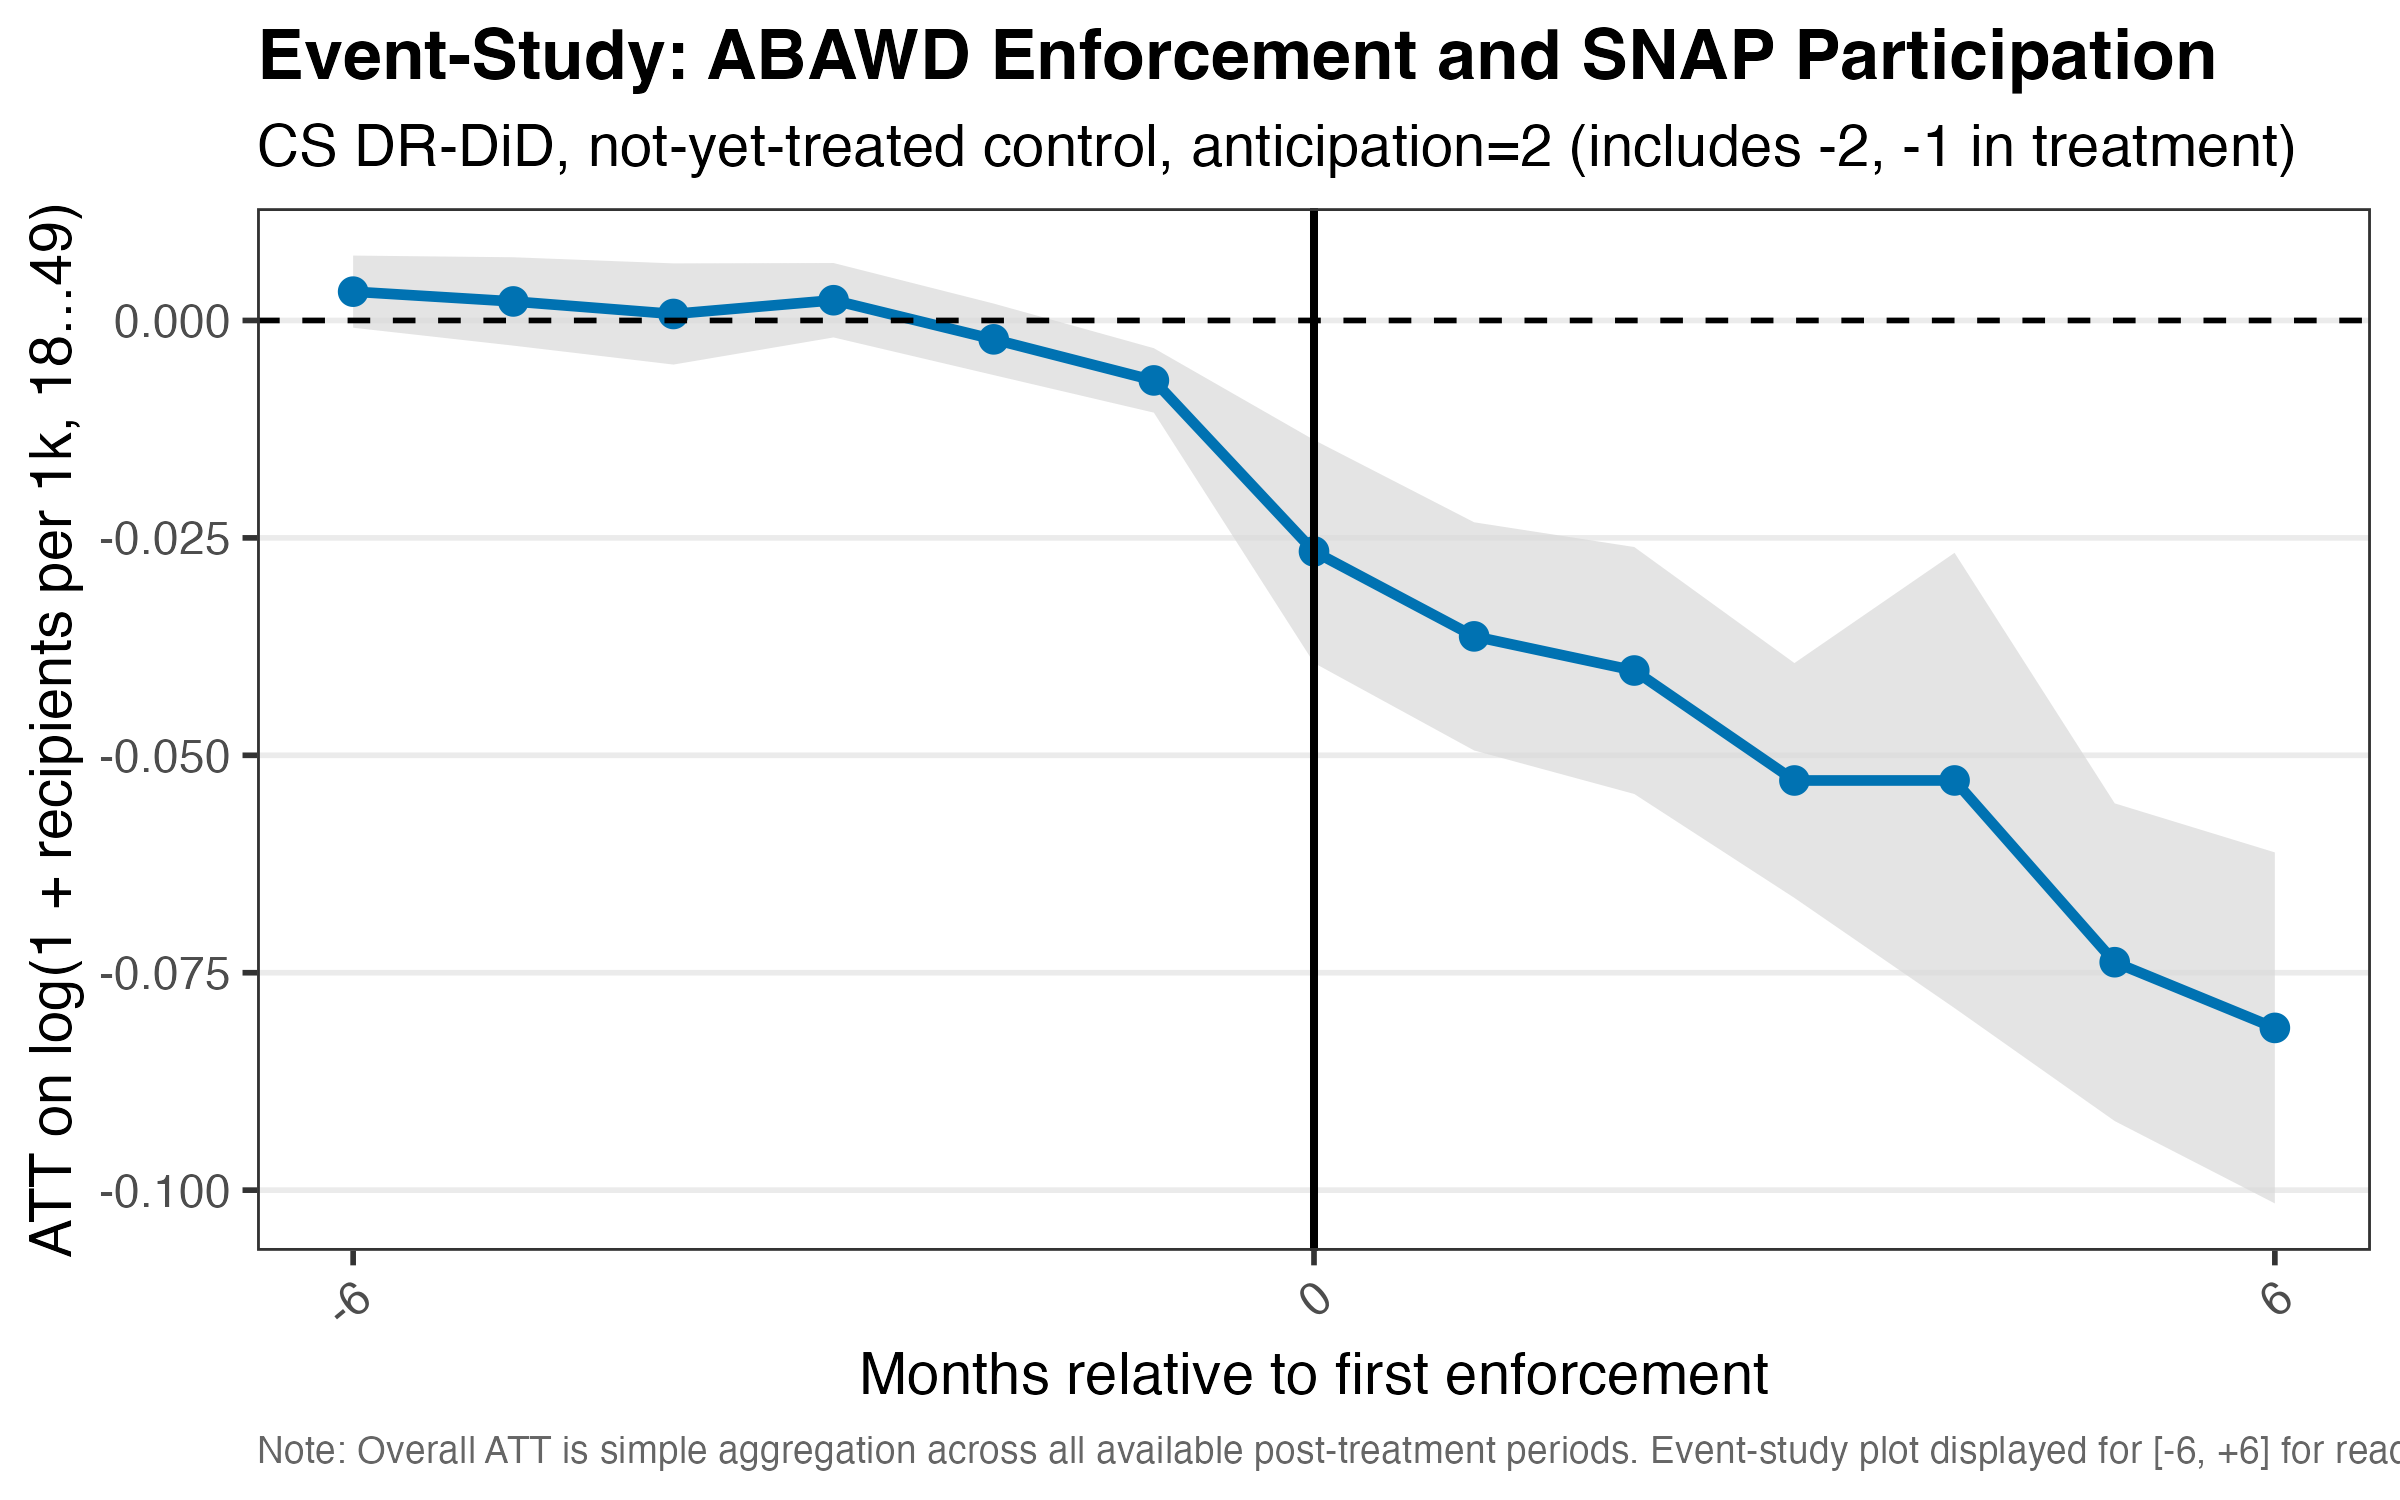
\includegraphics[width=0.85\textwidth]{../outputs/figures/abawd_es_main}
  \caption{Event-study: months relative to first ABAWD enforcement.}
  \label{fig:es_main}
\end{figure}

\subsection{DDD: adult vs.\ child}
\begin{figure}[htbp]
  \centering
  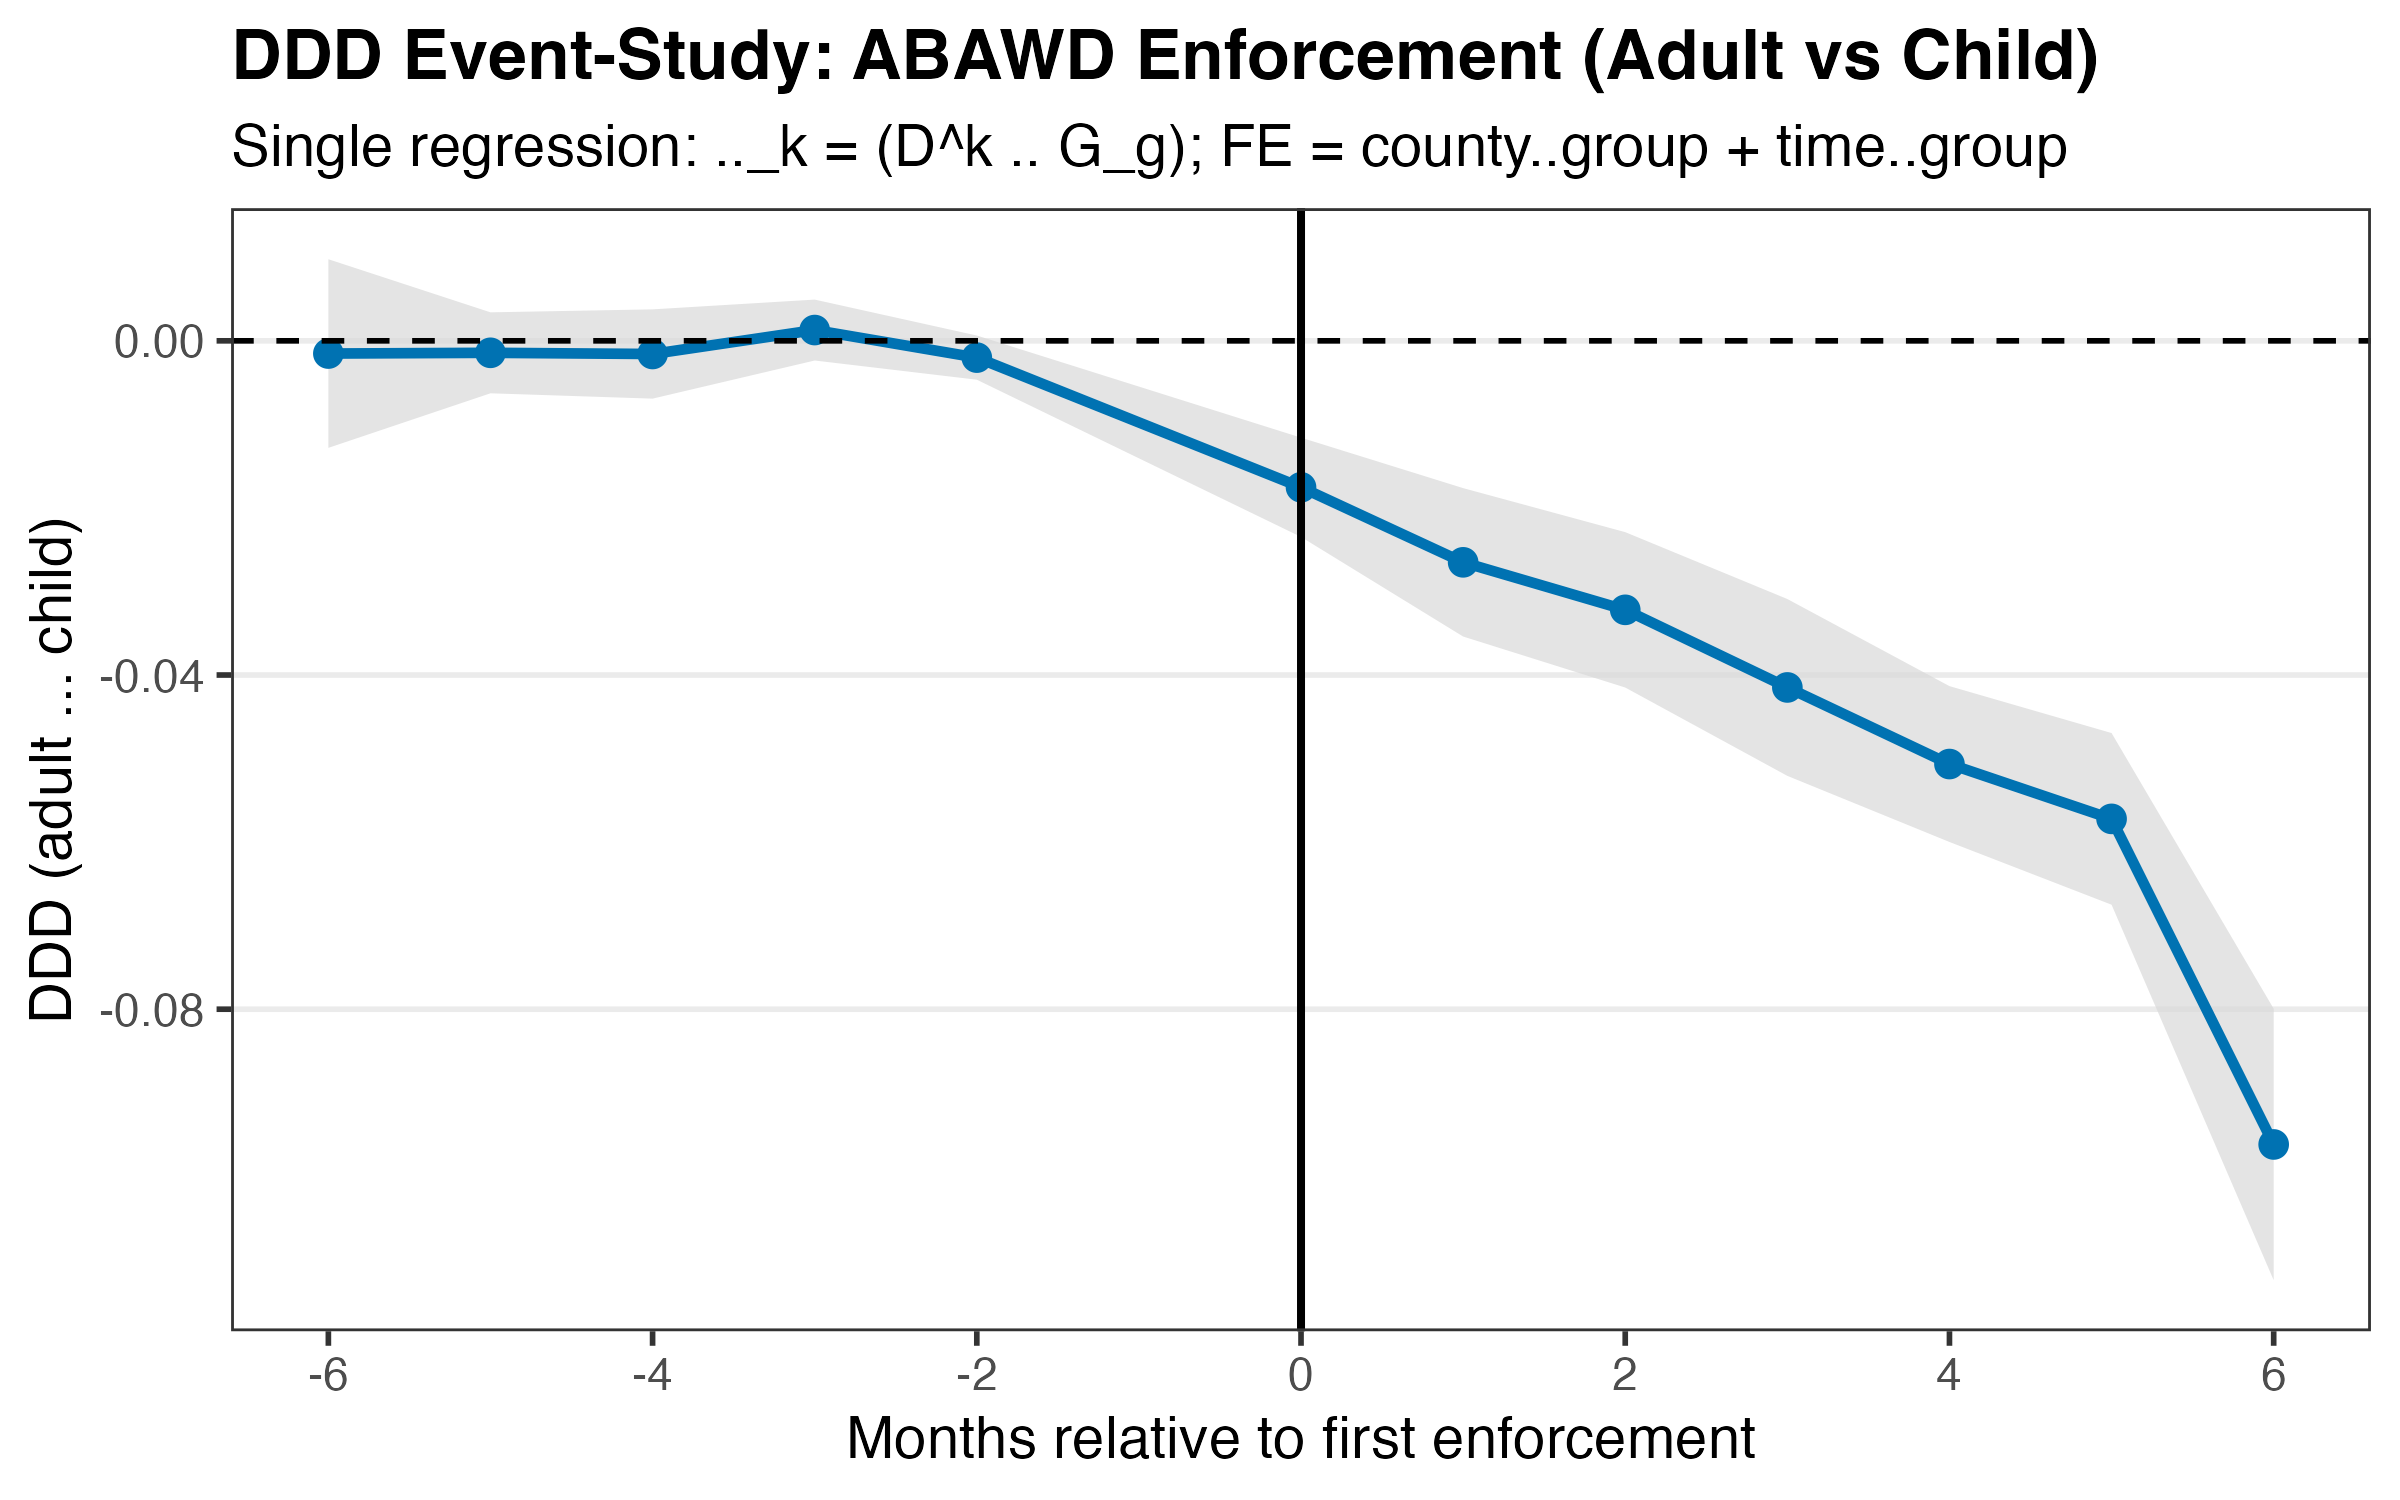
\includegraphics[width=0.85\textwidth]{../outputs/figures/abawd_es_ddd_adult_child}
  \caption{DDD event-study (adult minus child recipients).}
  \label{fig:ddd}
\end{figure}

\subsection{Heterogeneity: which counties were most affected?}
\begin{figure}[htbp]
  \centering
  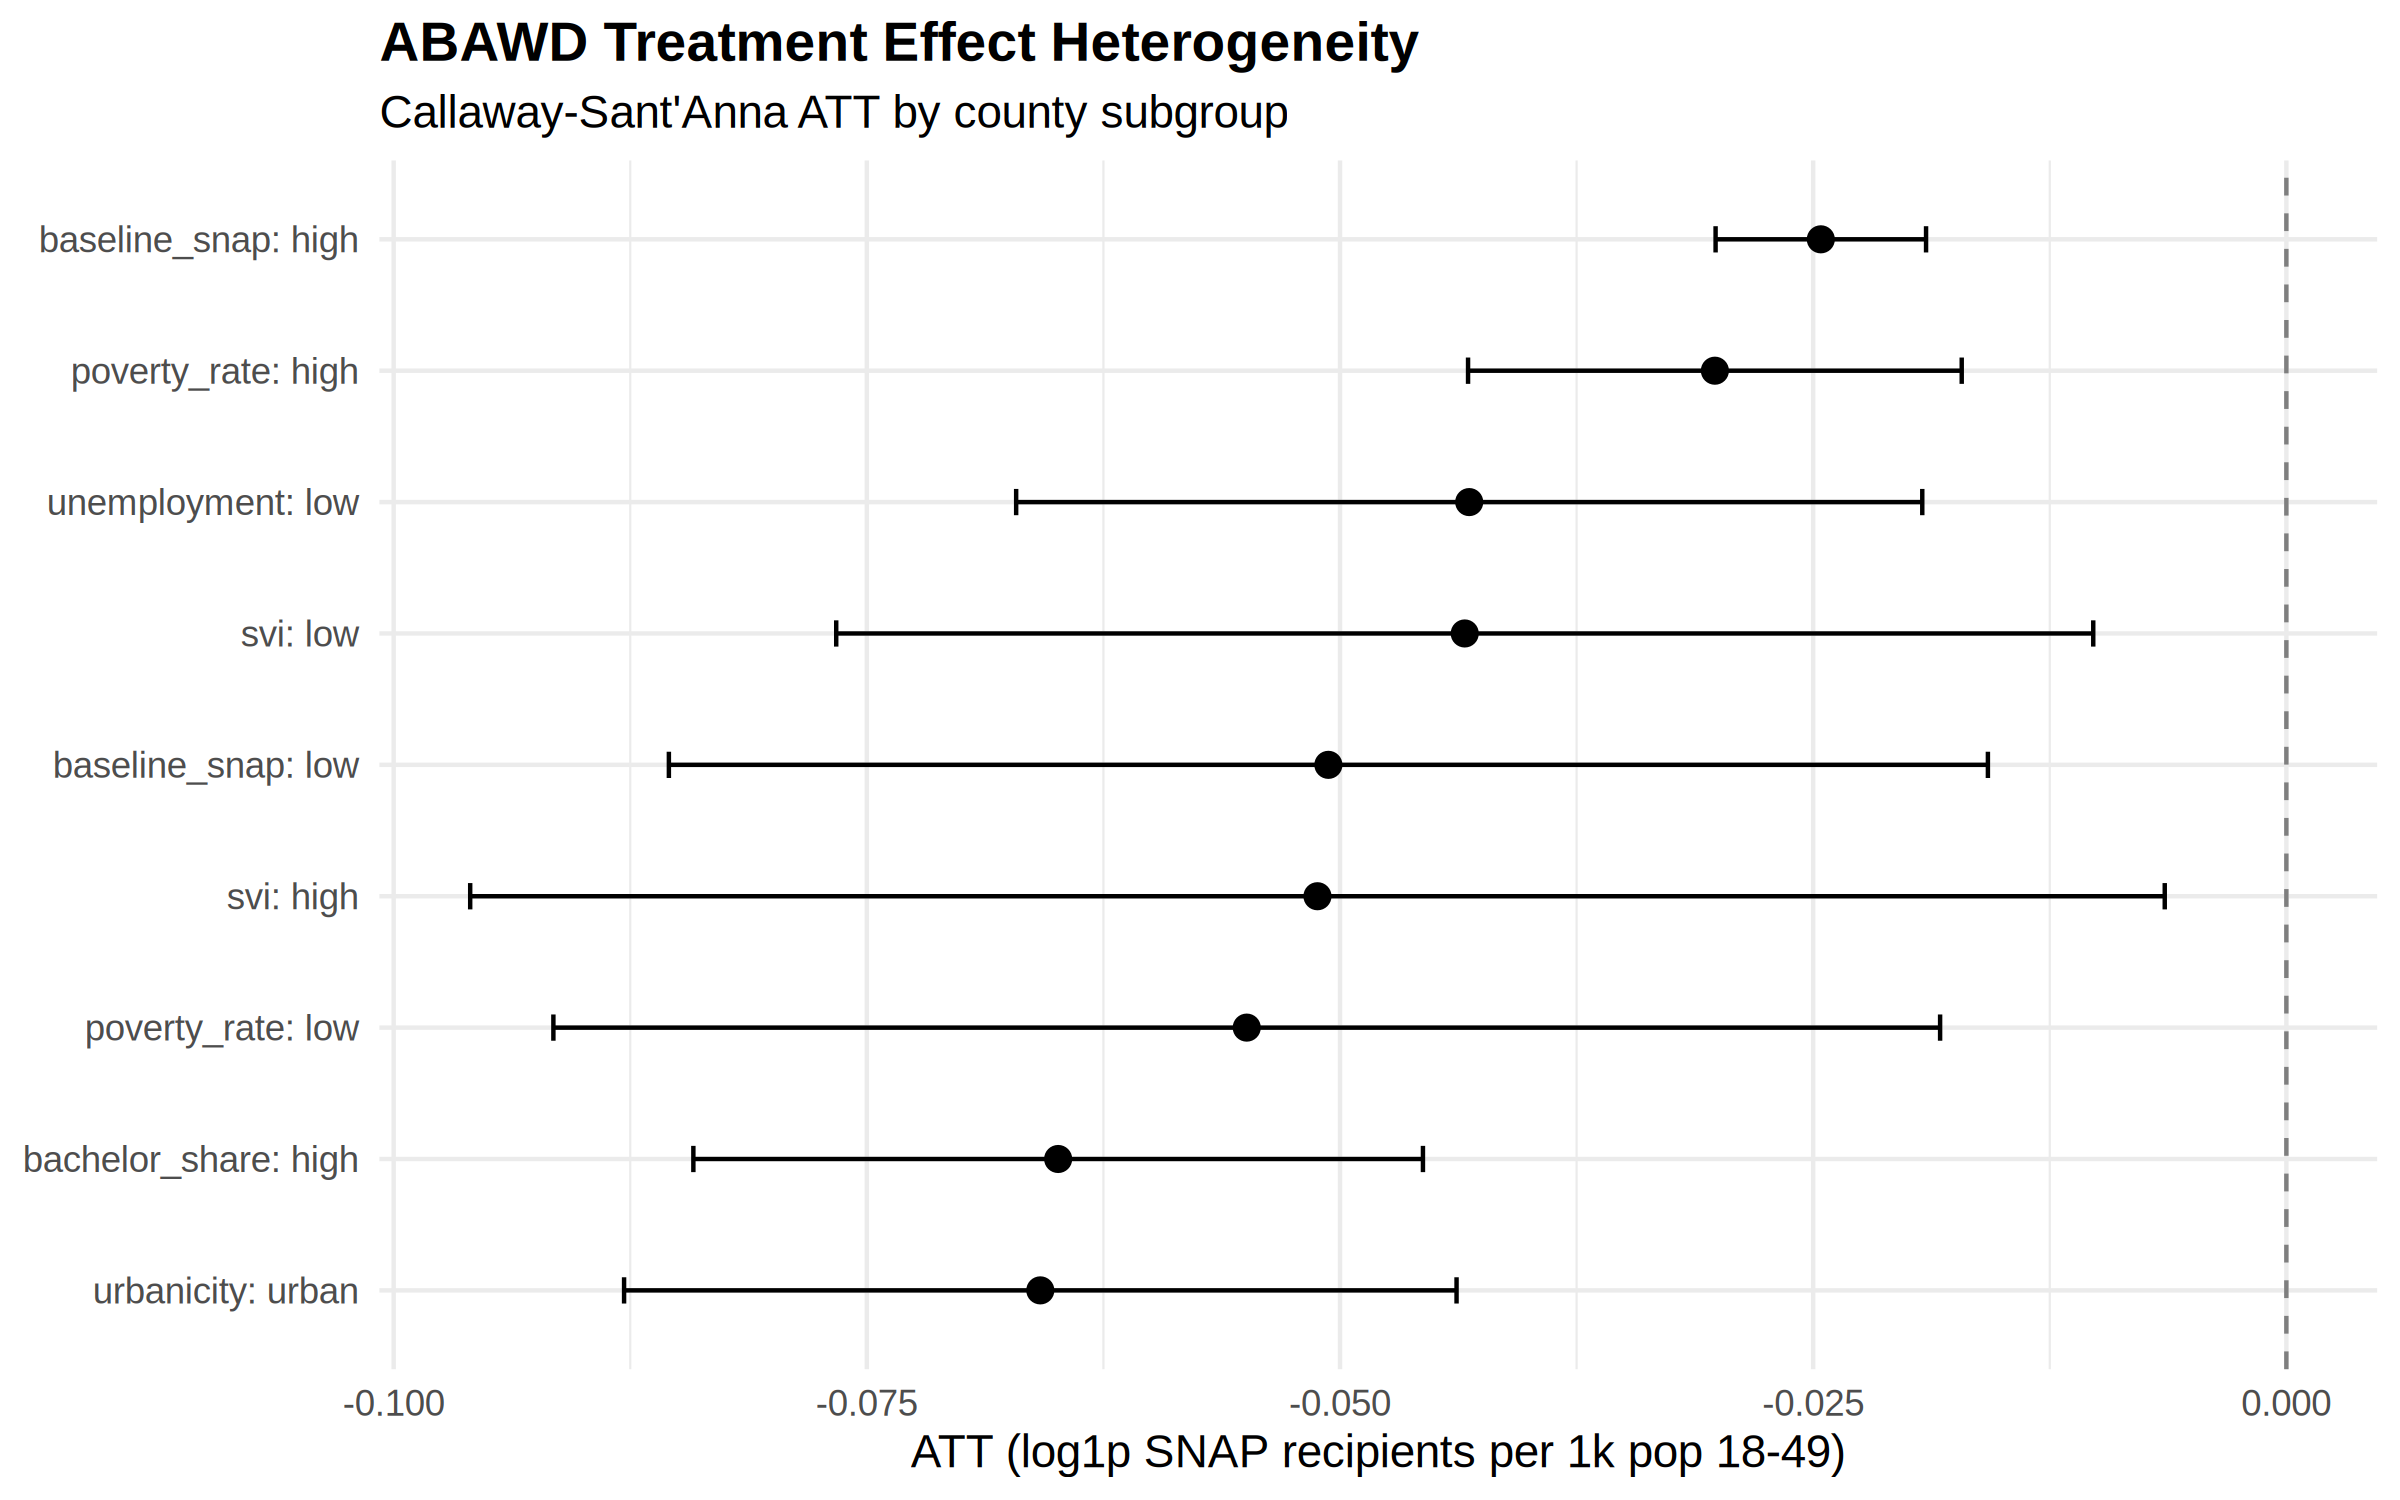
\includegraphics[width=0.85\textwidth]{../outputs/figures/abawd_heterogeneity_forest}
  \caption{ABAWD treatment effect heterogeneity by county subgroup.}
  \label{fig:het_forest}
\end{figure}

% Table: interaction coefficients from abawd_heterogeneity_interactions.csv
% Table: stabilizer correlation from abawd_stabilizer_correlation.csv

\subsection{County risk ranking under 2026 OBBA}
\begin{figure}[htbp]
  \centering
  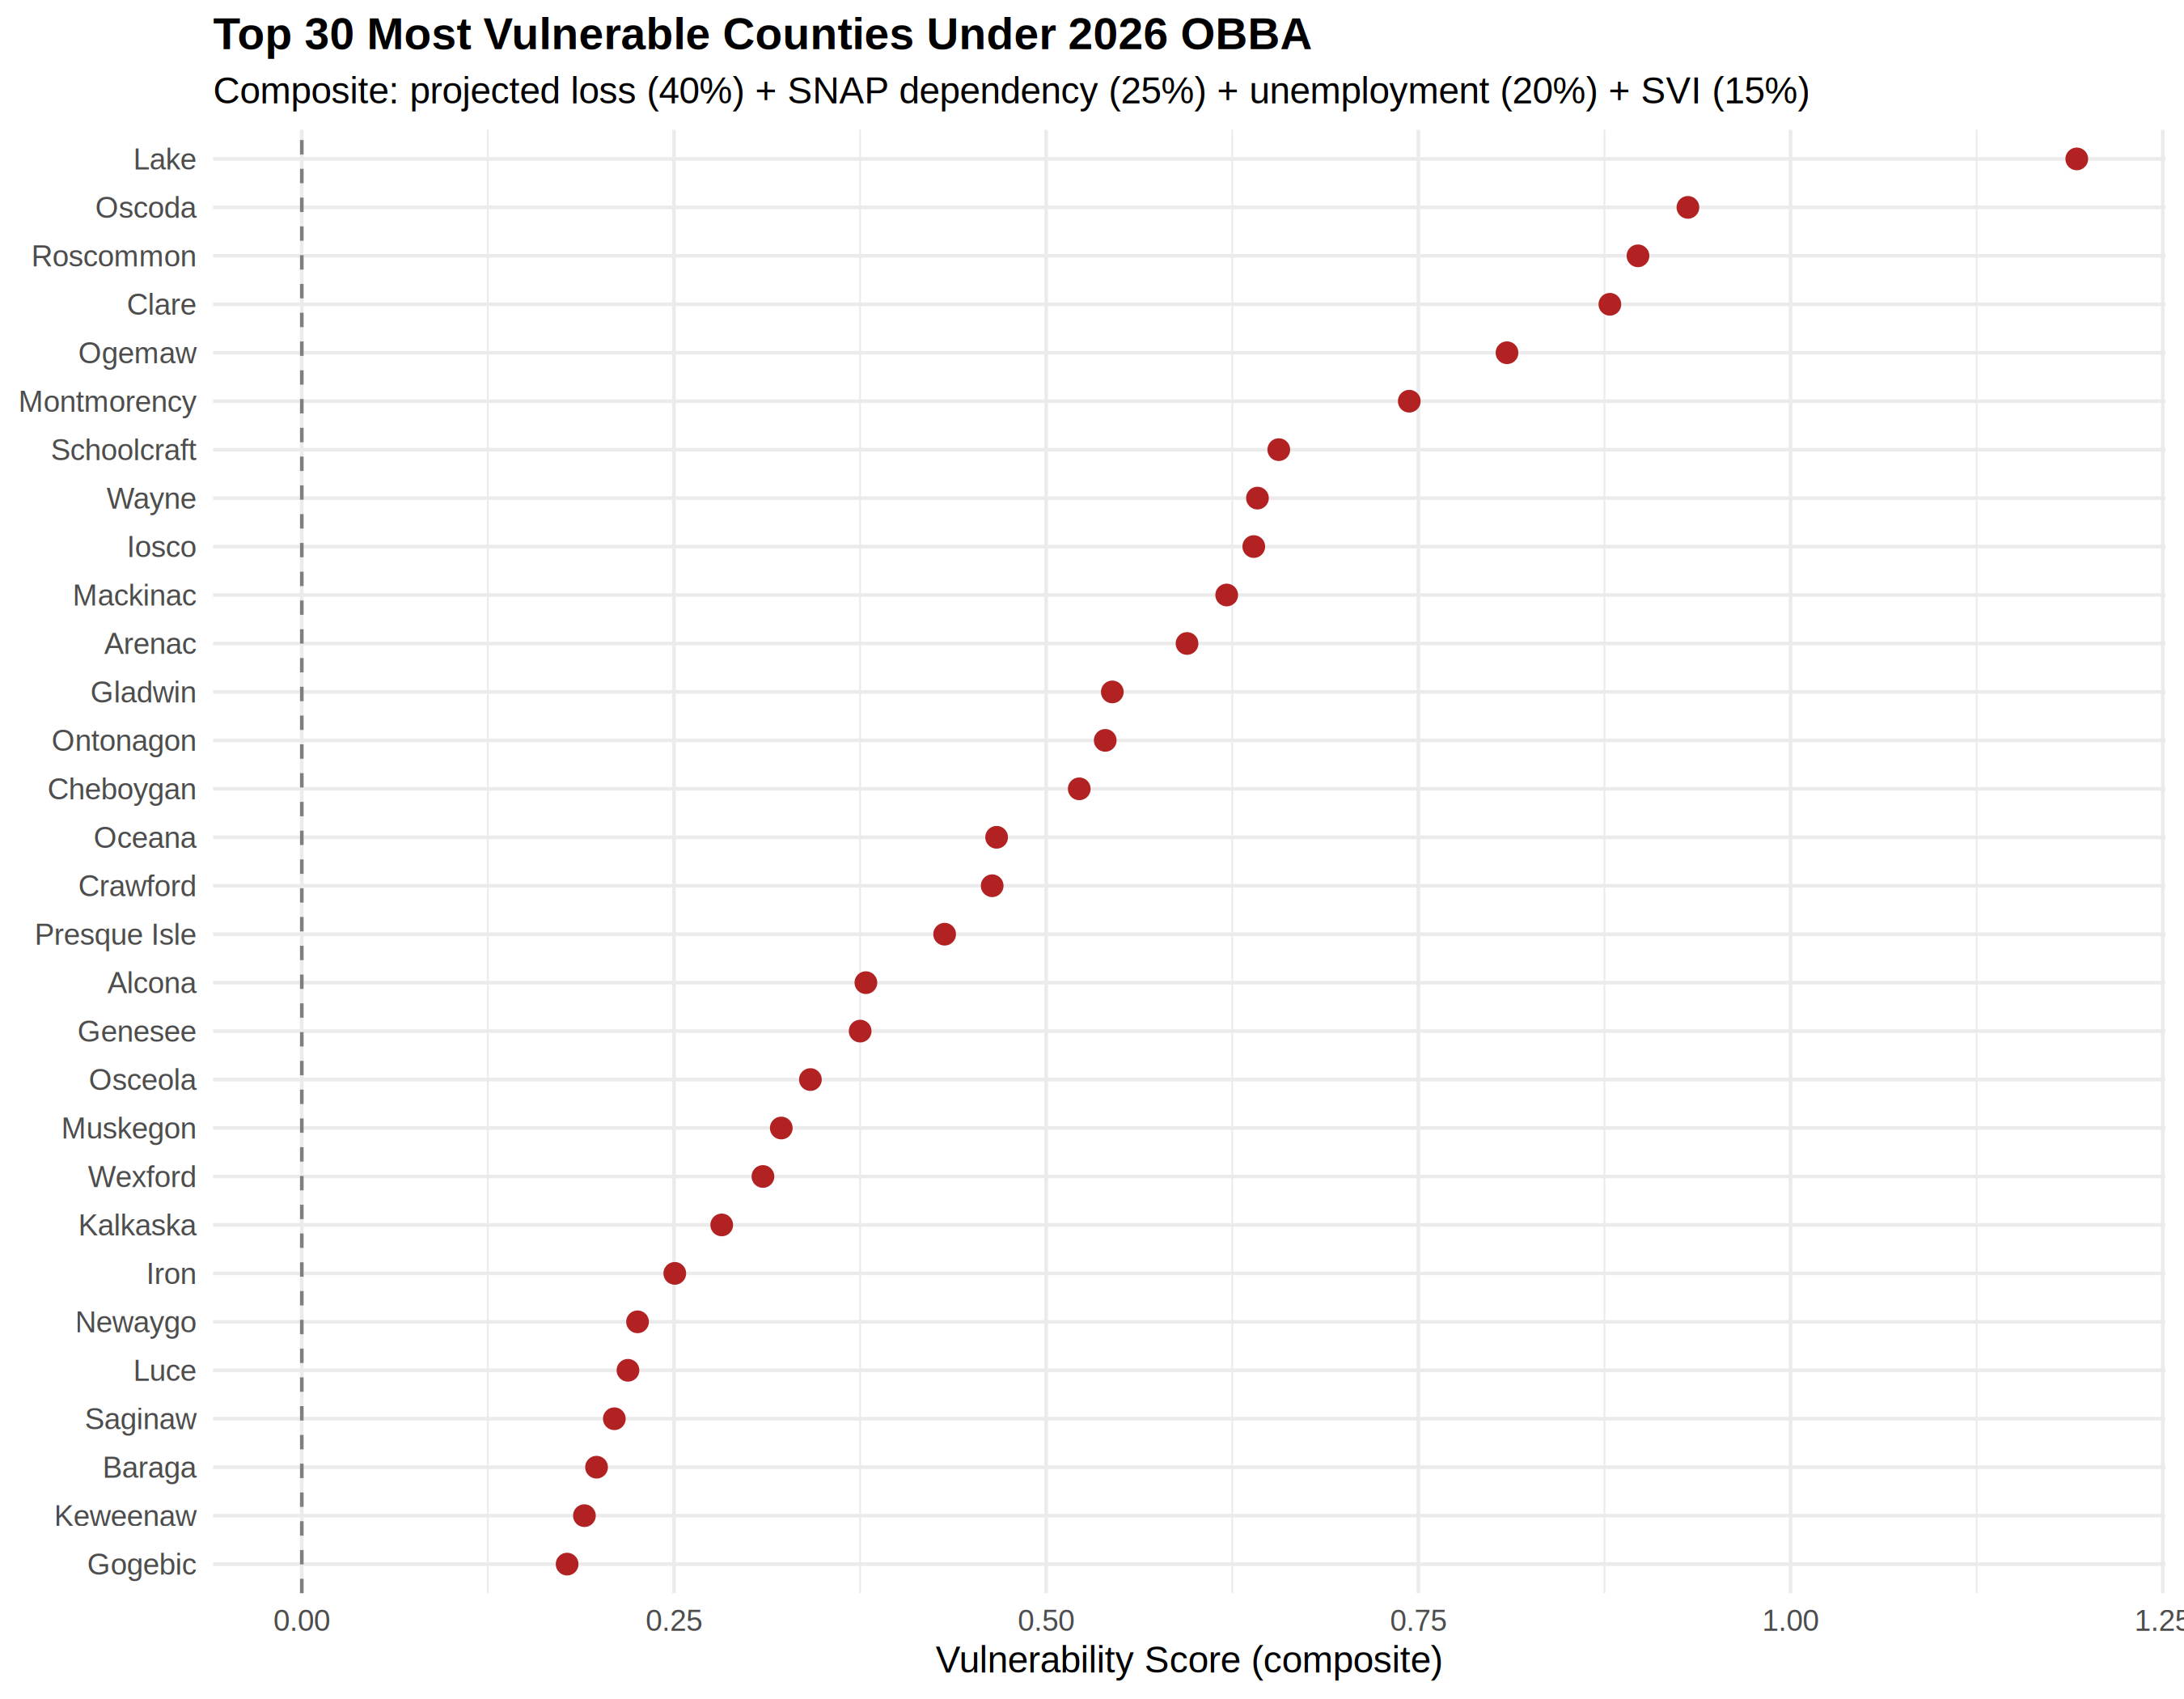
\includegraphics[width=0.85\textwidth]{../outputs/figures/vulnerability_ranking_dotplot}
  \caption{Top 30 most vulnerable counties under 2026 OBBA expansion.}
  \label{fig:vuln_dotplot}
\end{figure}

\IfFileExists{../outputs/figures/vulnerability_map.png}{%
\begin{figure}[htbp]
  \centering
  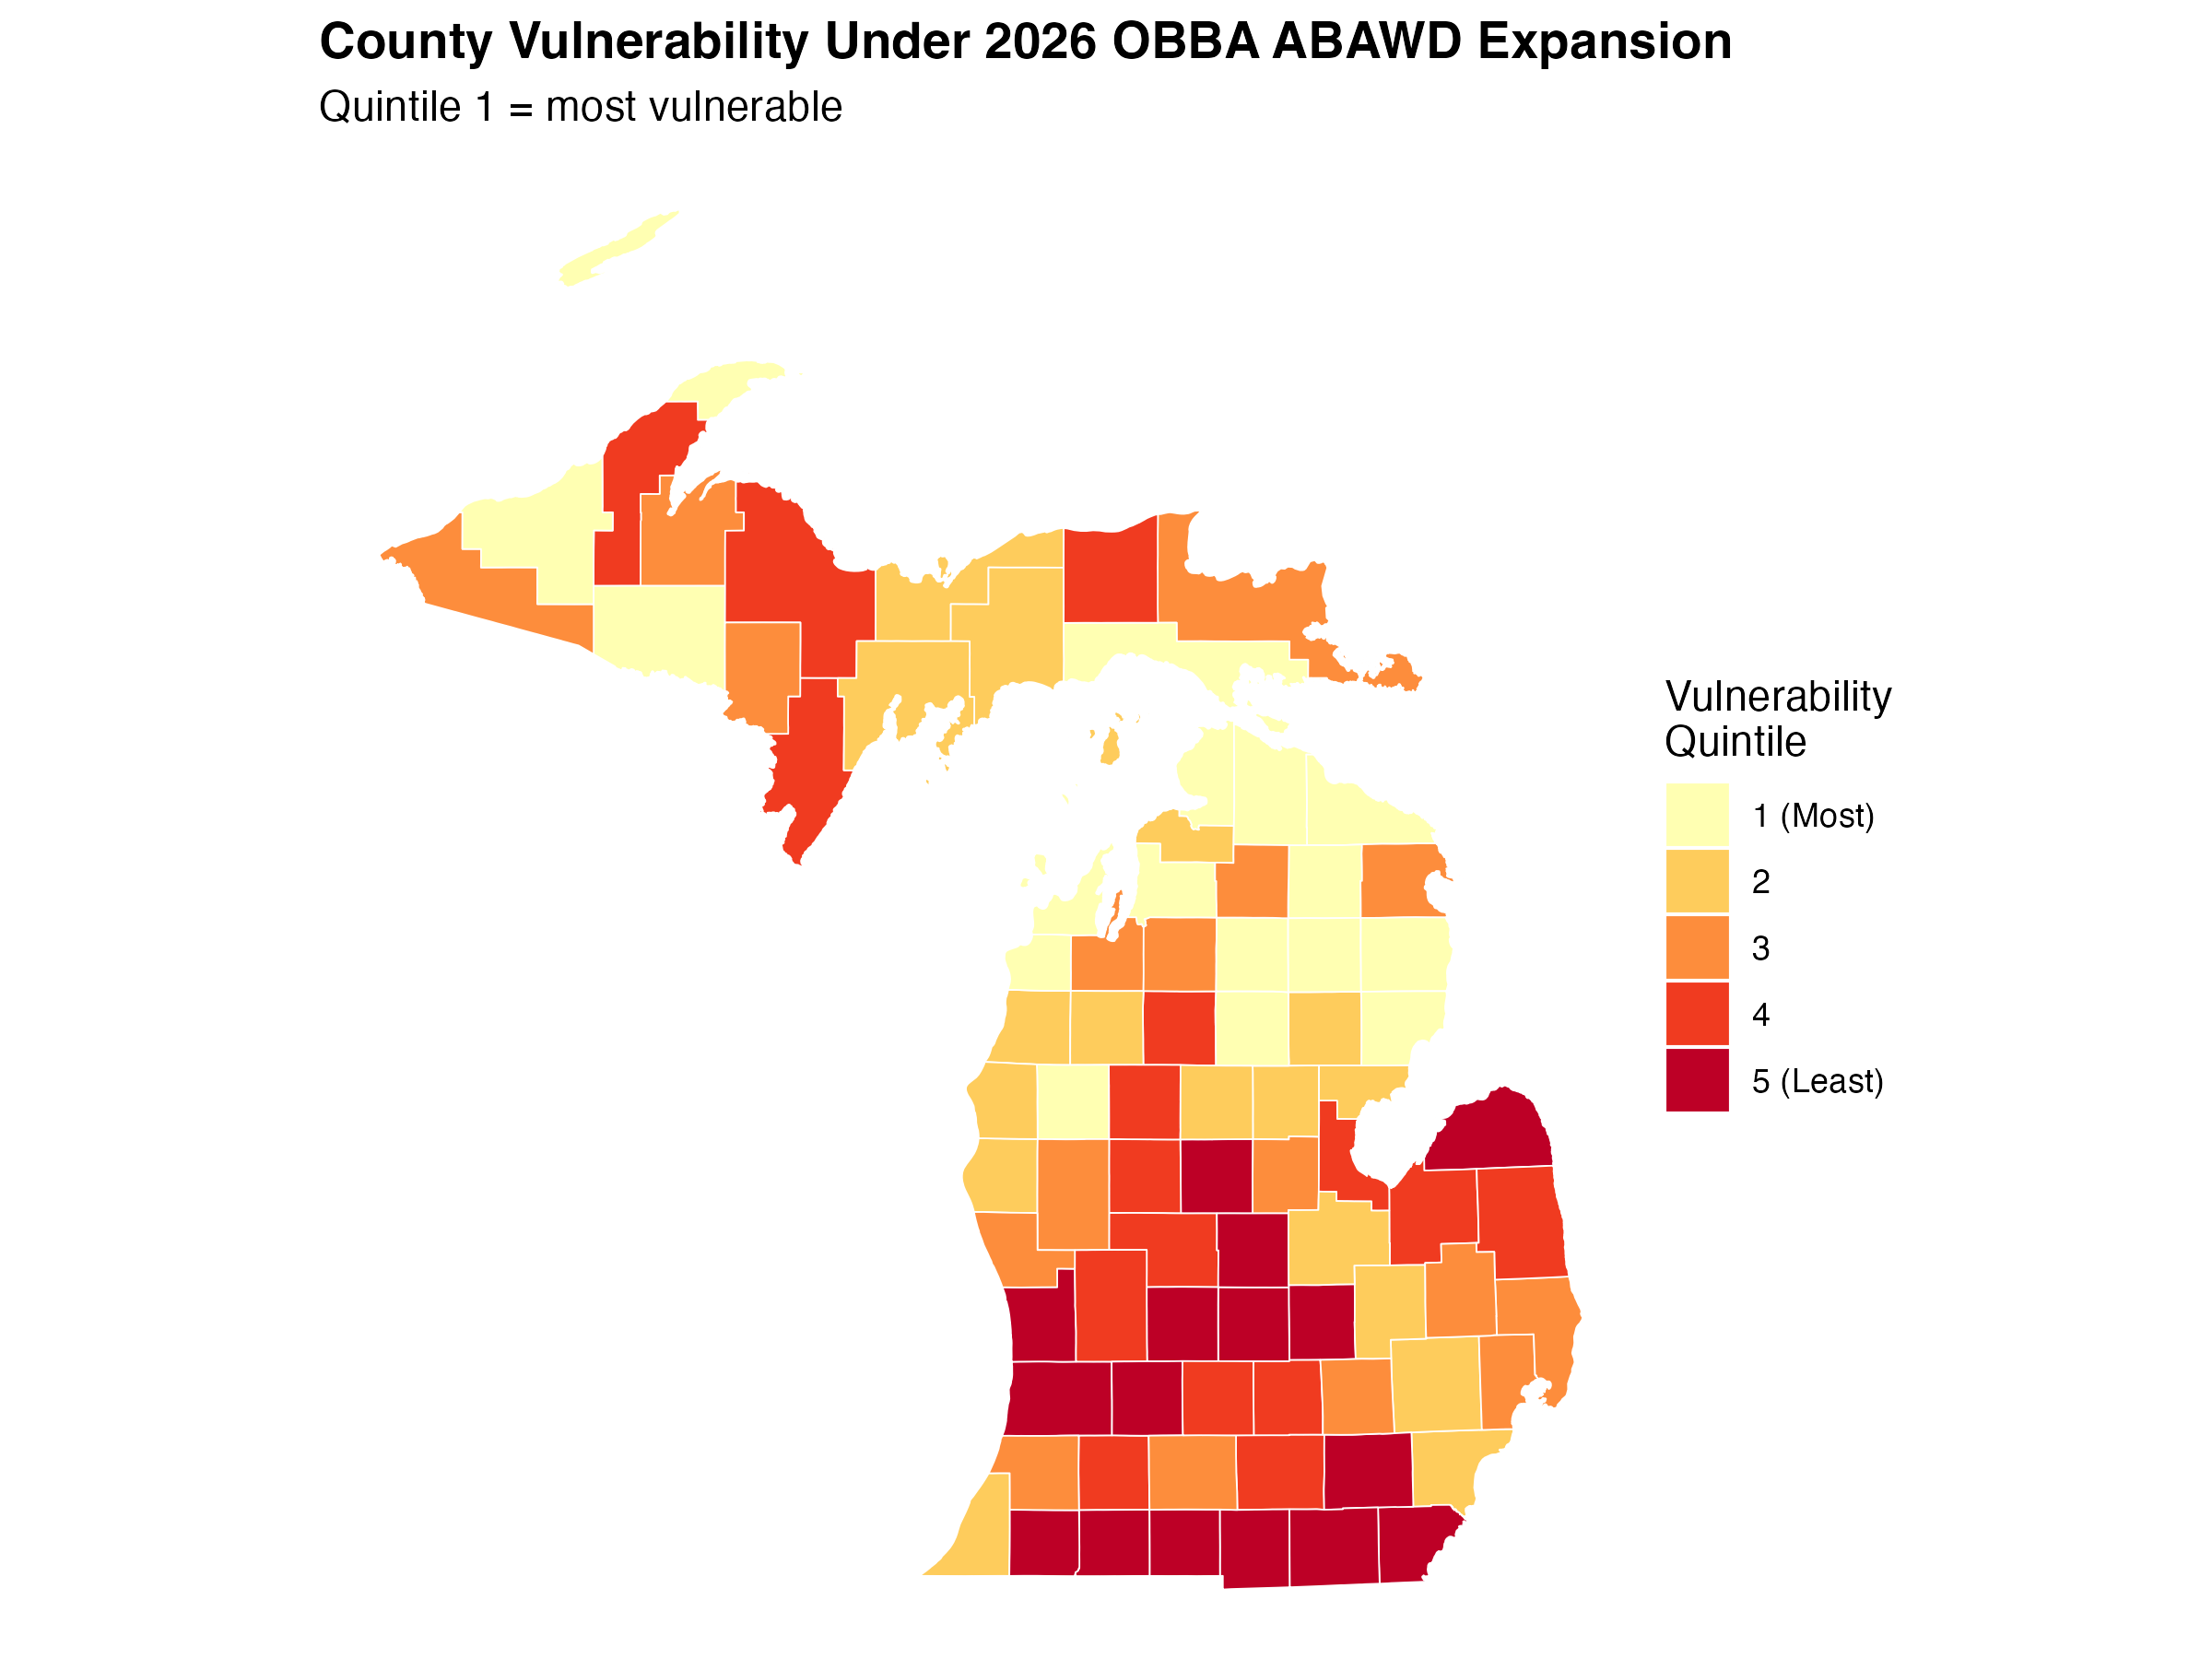
\includegraphics[width=0.7\textwidth]{../outputs/figures/vulnerability_map}
  \caption{Michigan county vulnerability map (quintiles).}
  \label{fig:vuln_map}
\end{figure}
}{}

% Table: forecast_2026_summary.csv (state-level totals, 3 scenarios, CI)
% Table: county_vulnerability_ranking.csv (top 20 counties with scores)

\subsection{Automatic stabilizer interpretation}
\begin{figure}[htbp]
  \centering
  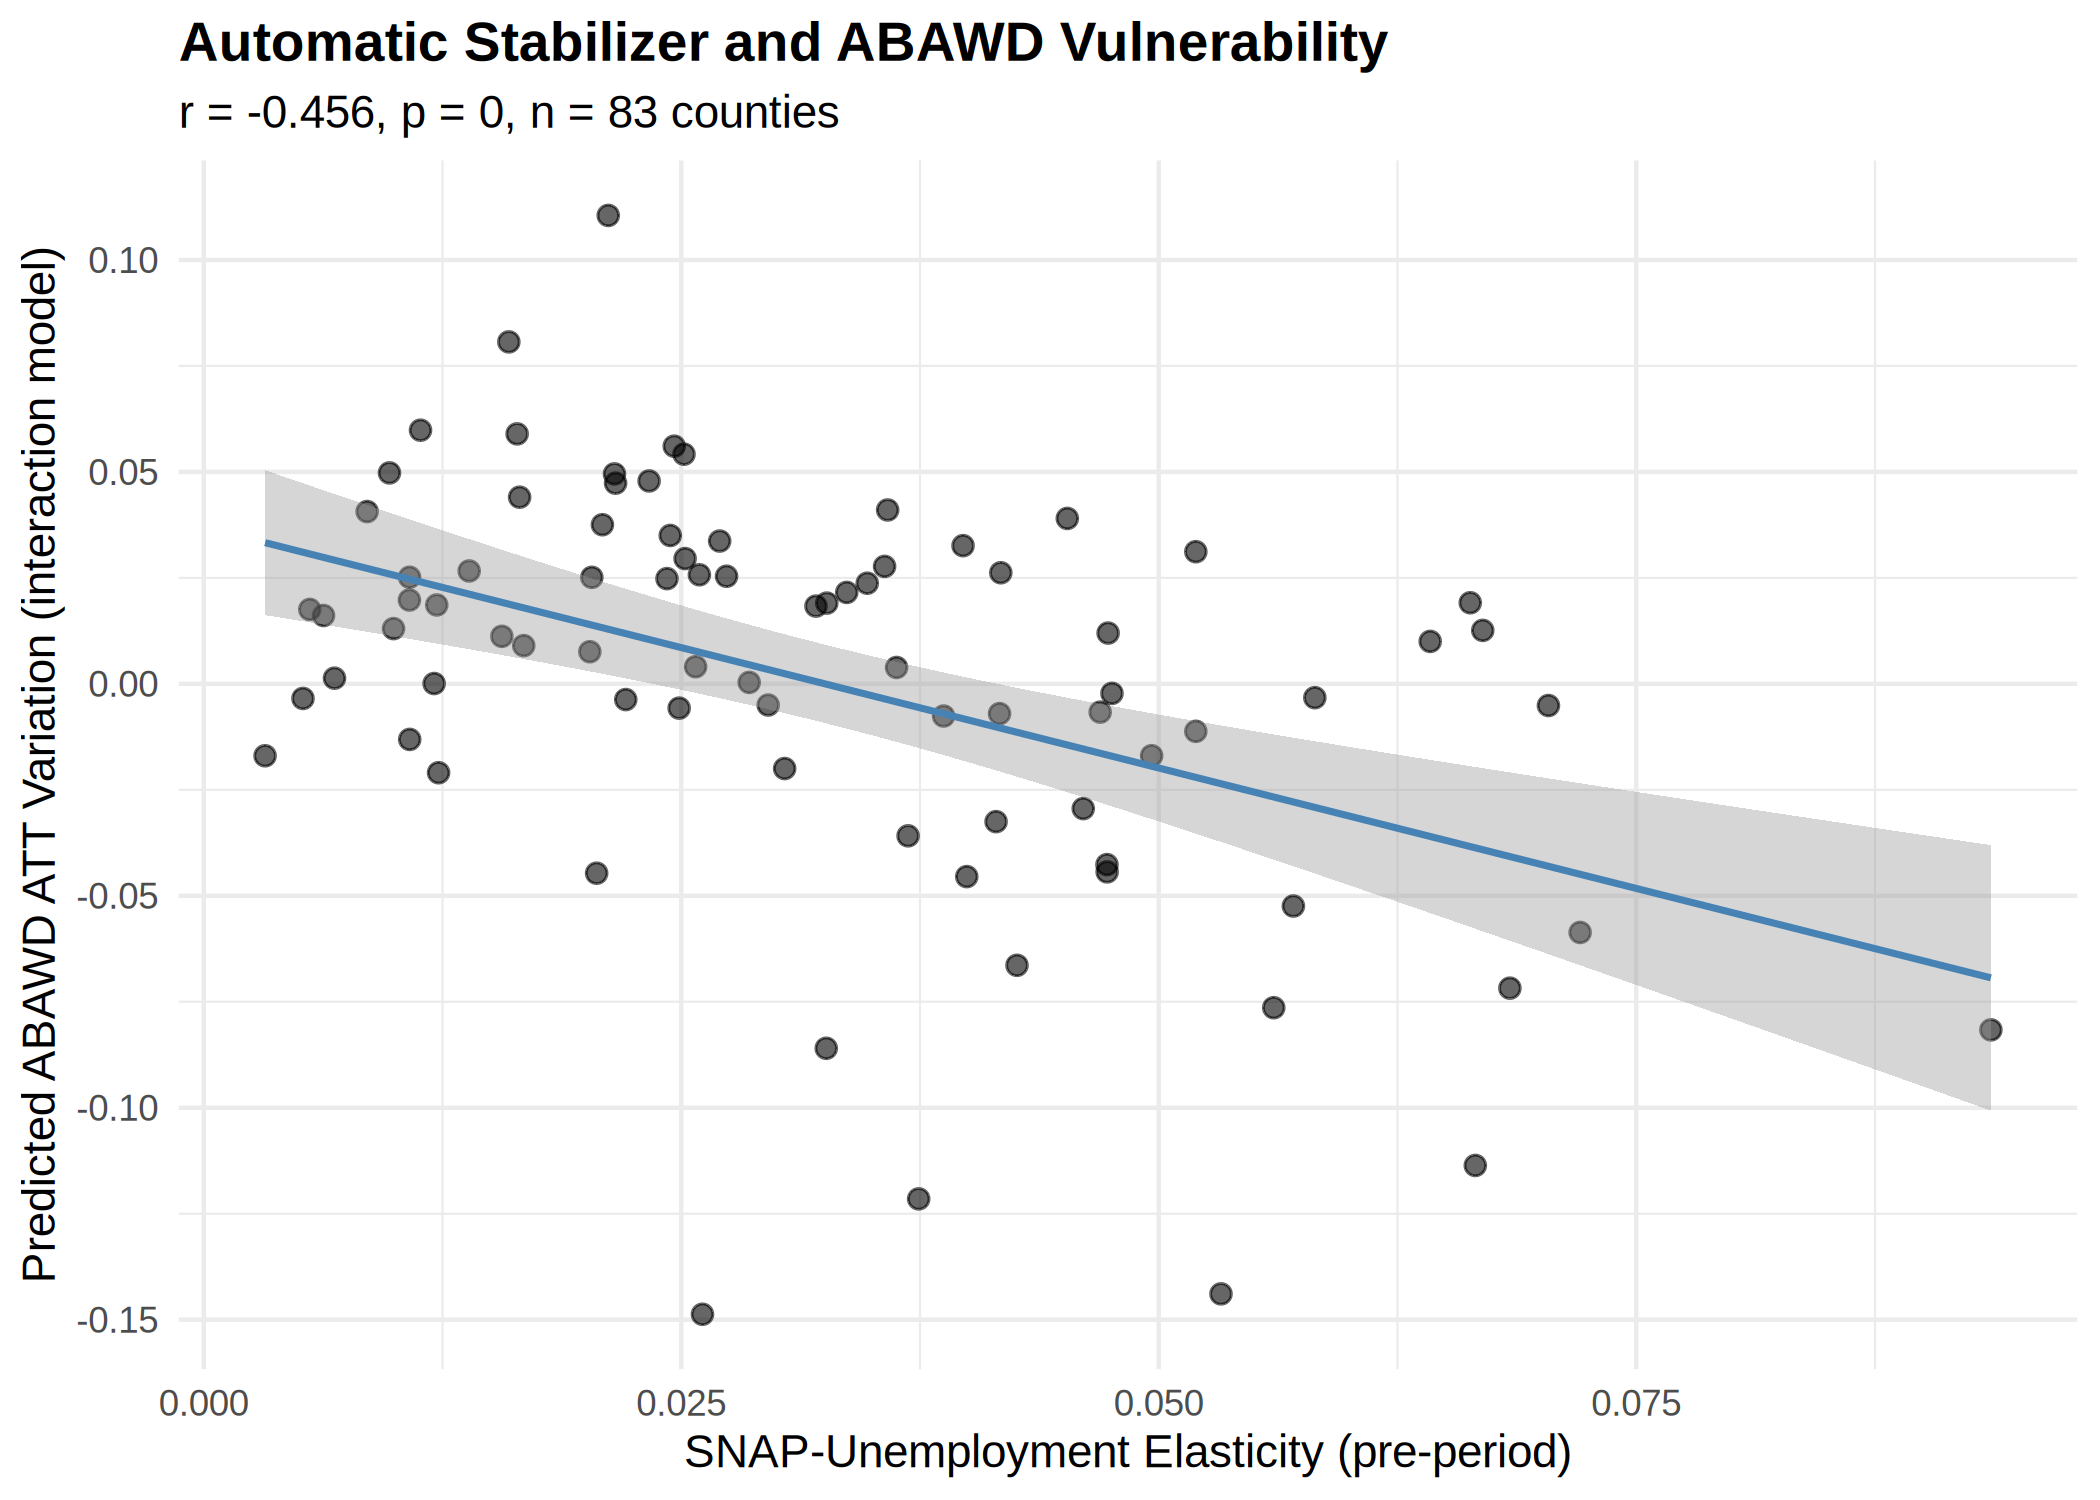
\includegraphics[width=0.7\textwidth]{../outputs/figures/abawd_stabilizer_scatter}
  \caption{SNAP-unemployment elasticity vs.\ predicted ABAWD treatment effect variation.}
  \label{fig:stabilizer}
\end{figure}

\section{Discussion and Policy Implications}
\label{sec:discussion}
% Which counties need targeted outreach?
% Administrative capacity constraints
% Limitations: county-level, no individual mechanisms
% External validity: Michigan reinstatement → future expanded policy

\section{Conclusion}
\label{sec:conclusion}

\bibliographystyle{plain}
\bibliography{refs}
\end{document}
